\newpage 
\chapter{آنتن آرایه ای ، تزویج ( کوپلینگ ) و راه های کاهش آن}
\label{ch:2}
\section{مقدمه}
پس از آشنایی با اصول طراحی و تحلیل آنتن‌های مایکرواستریپ تکی، در این فصل به بررسی آرایه‌های آنتن و چالش‌های مرتبط با تزویج متقابل
\LTRfootnote{Coupling}
 بین المان‌های آرایه پرداخته می‌شود. هدف اصلی، تبیین مکانیزم‌های تزویج و ارائه راه‌کارهای عملی برای کاهش اثرات نامطلوب آن در عملکرد آرایه است.
 
\section{آرایه ها و شبکه ی تغذیه}
آرایهٔ آنتنی به مجموعه‌ای از چندین المان تشعشعی گفته می‌شود که به صورت منظم یا نامنظم در کنار یکدیگر قرار گرفته و با تغذیهٔ مناسب، الگوی تشعشعی دلخواه ایجاد می‌کنند. آرایه‌ها معمولاً از ترکیب آنتن‌های ساده‌ای مانند پچ، دیپل یا شکاف ساخته می‌شوند و با تنظیم دامنه و فاز جریان تغذیهٔ هر المان، می‌توان شکل پرتو را کنترل و در جهات مختلف هدایت کرد.


آرایه‌ها کاربردپذیری بالایی دارند و برای تولید الگوهای تشعشعی مورد نظر که با یک المان منفرد قابل دستیابی نیستند، استفاده می‌شوند. به علاوه، برای چرخاندن پرتو یک سیستم آنتن، افزایش سمت‌گرایی
\LTRfootnote{Directivity}
 و انجام کارهایی که با المان‌های تکی دشوار است، به‌کار گرفته می‌شوند. به همین دلیل، آرایه‌ها نقش کلیدی در رادارها، سیستم‌های مخابرات ماهواره‌ای،
 \lr{5G}
  و سامانه‌های
  \lr{MIMO}
   ایفا می‌کنند.
   
   
   آرایه ها به دو صورت میتوانند تغذیه شوند:‌ تغذیه ی سری و موازی. البته به صورت ترکیبی هم ممکن است.
   

\begin{figure}[t]
	\centering
	\begin{subfigure}{0.3\textwidth} % width of left subfigure
		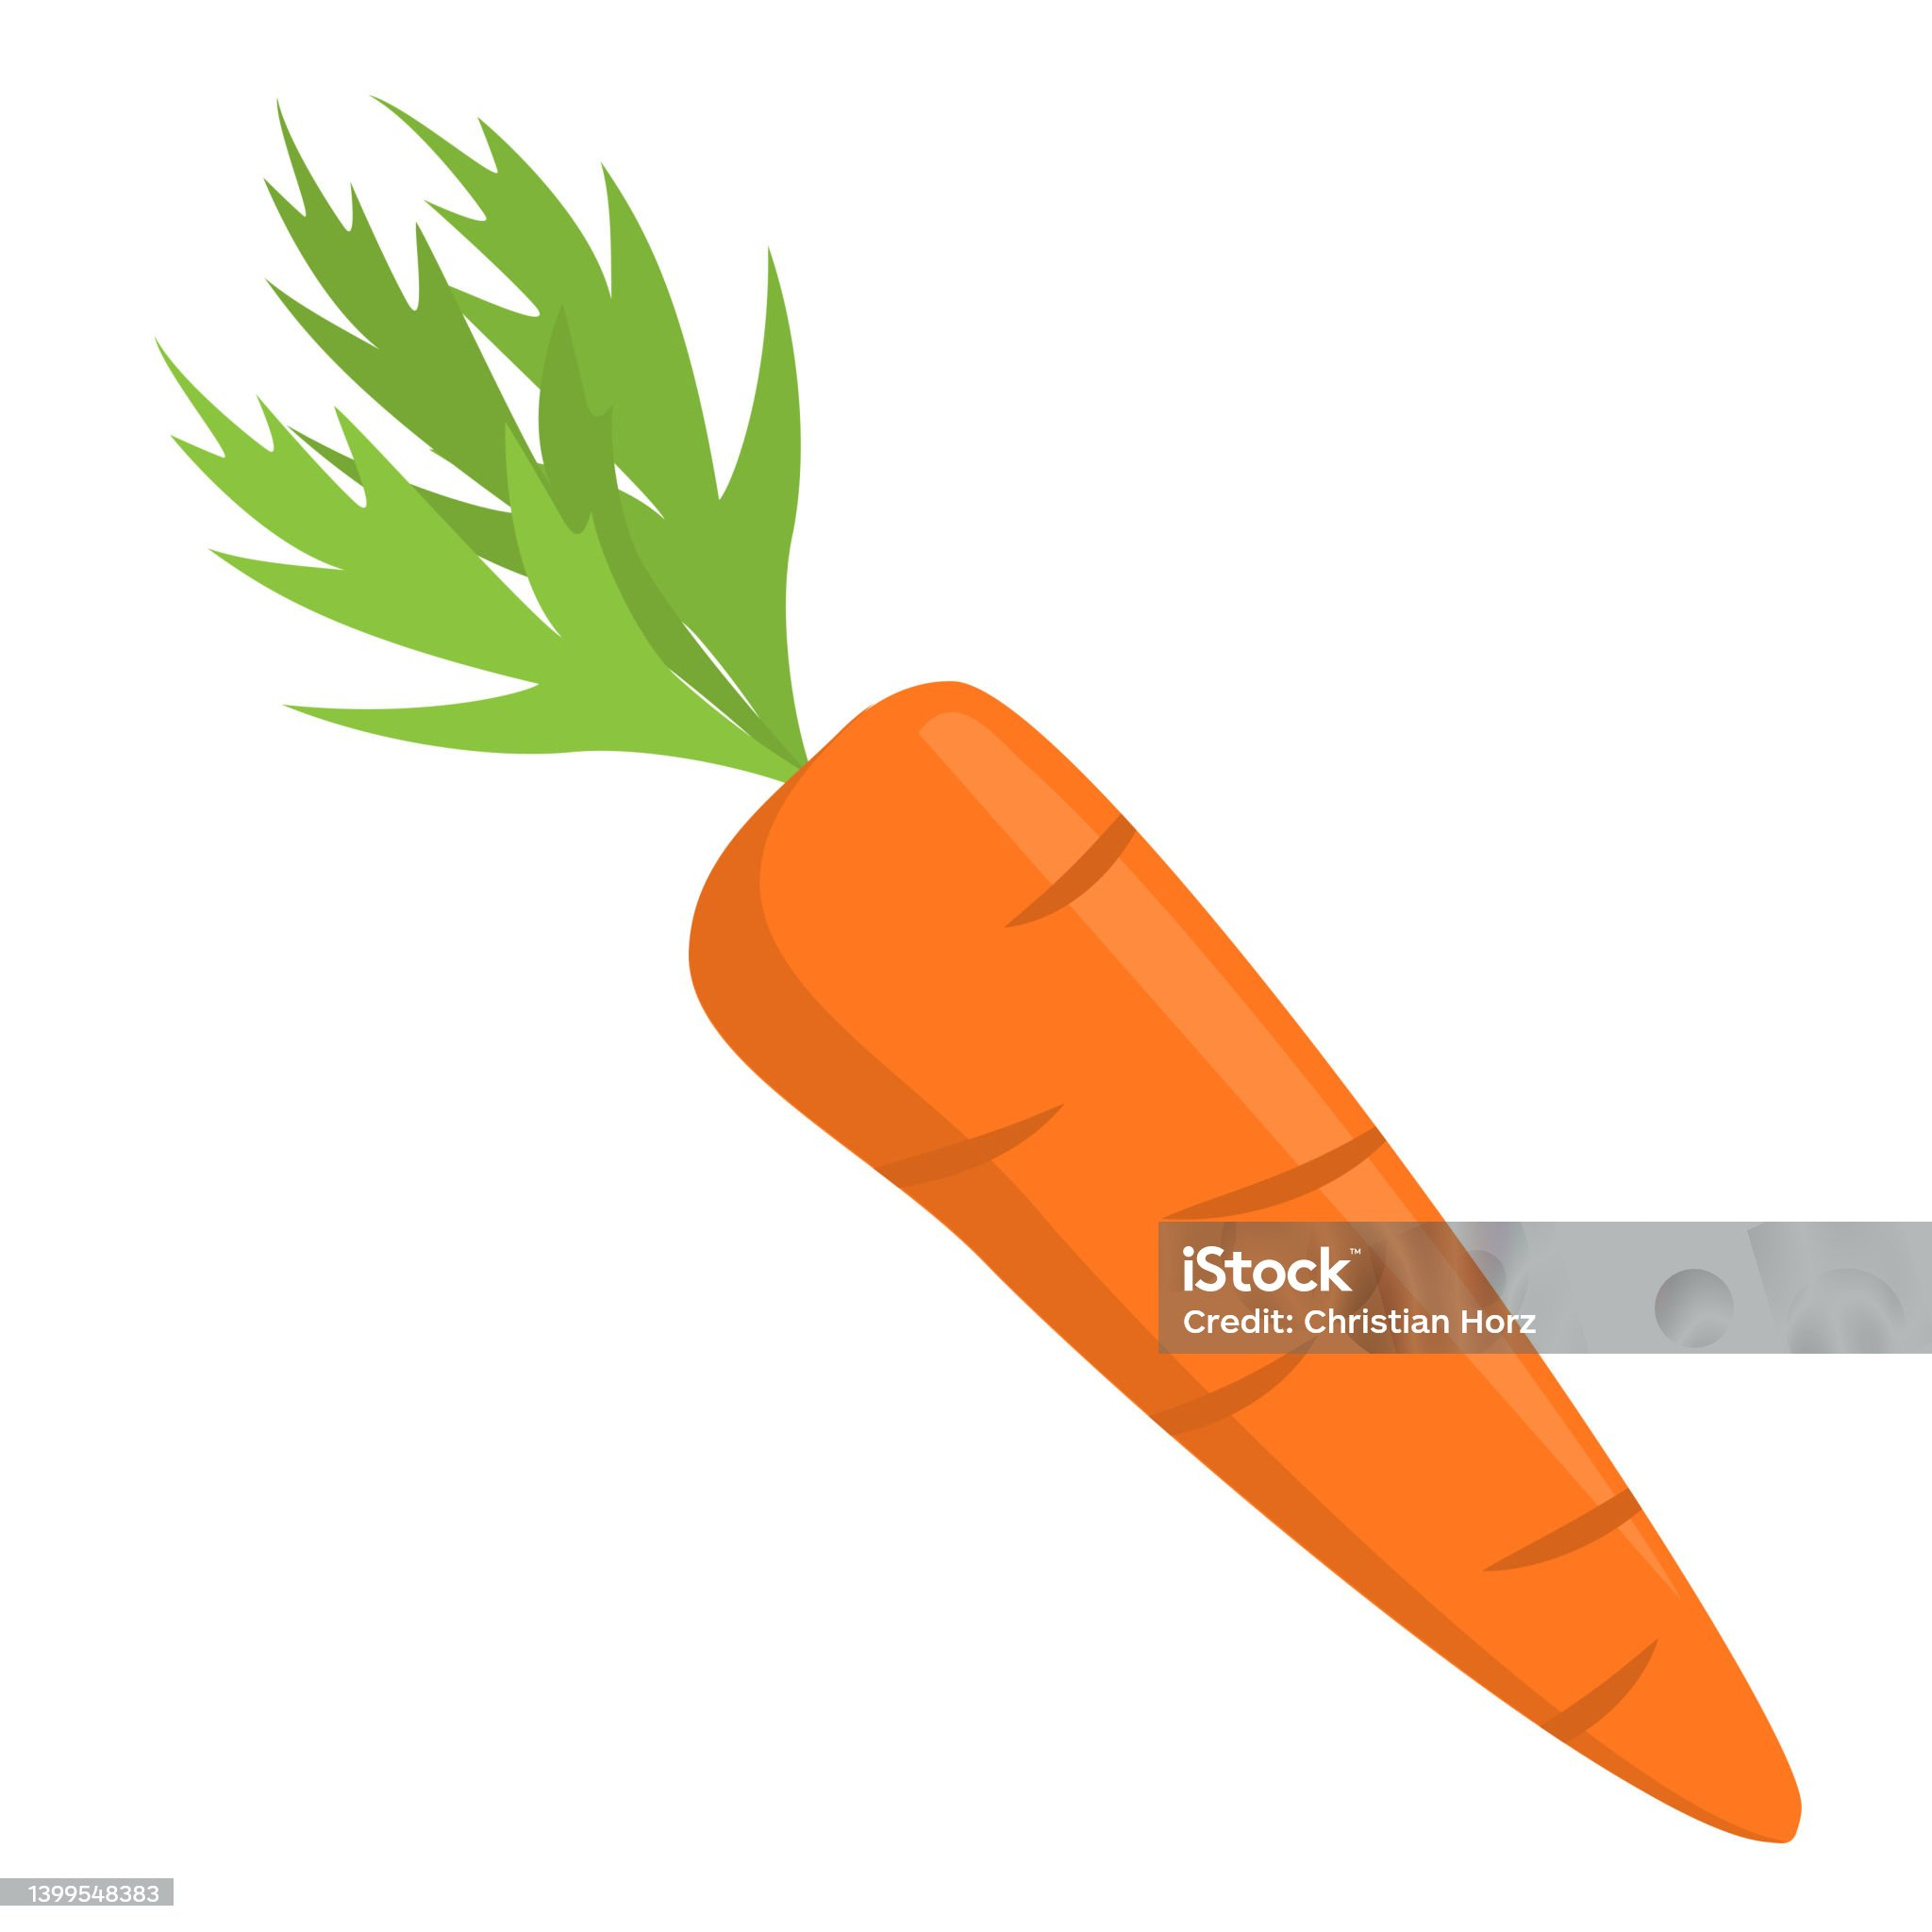
\includegraphics[scale=0.2]{Images/aaa.jpg}
		\caption{تغذیه سری} % subcaption
		\label{fig12}
	\end{subfigure}
	\vspace{1em} % here you can insert horizontal or vertical space
	\begin{subfigure}{0.3\textwidth} % width of right subfigure
		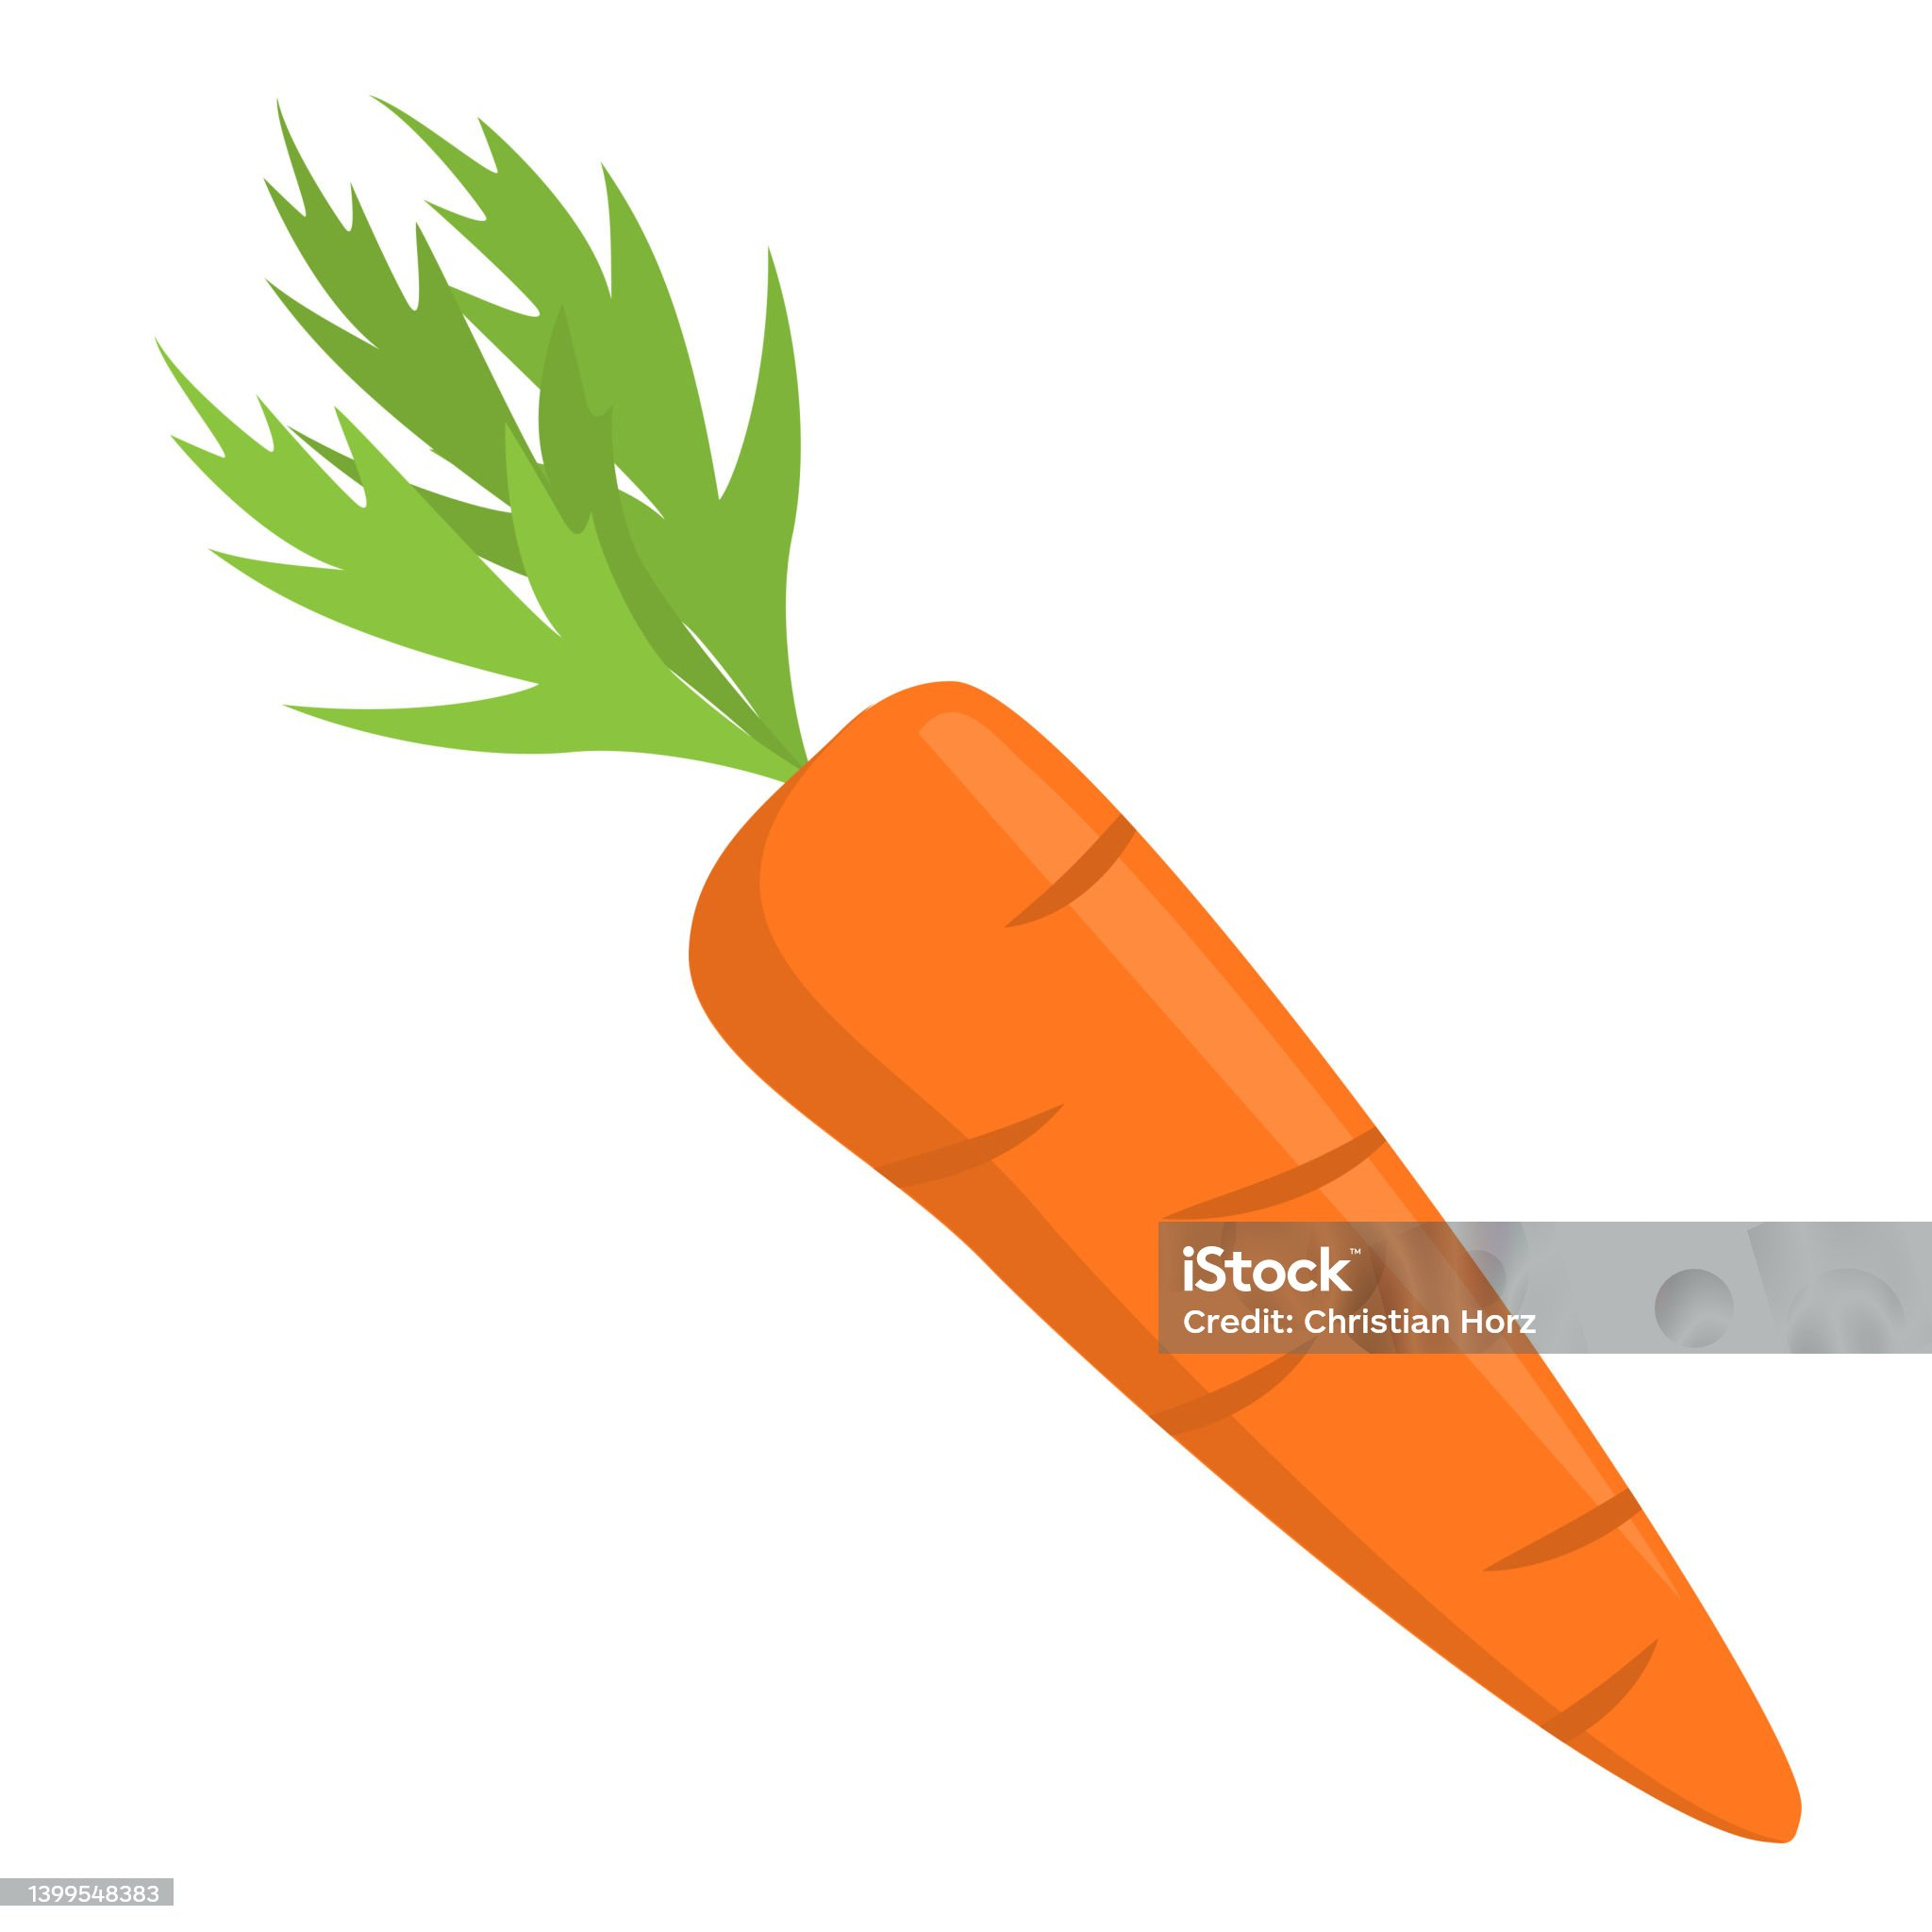
\includegraphics[scale=0.2]{Images/aaa.jpg}
		\caption{تغذیه موازی} % subcaption
		\label{fig13}
	\end{subfigure}
		\vspace{1em} % here you can insert horizontal or vertical space
	\begin{subfigure}{0.3\textwidth} % width of right subfigure
		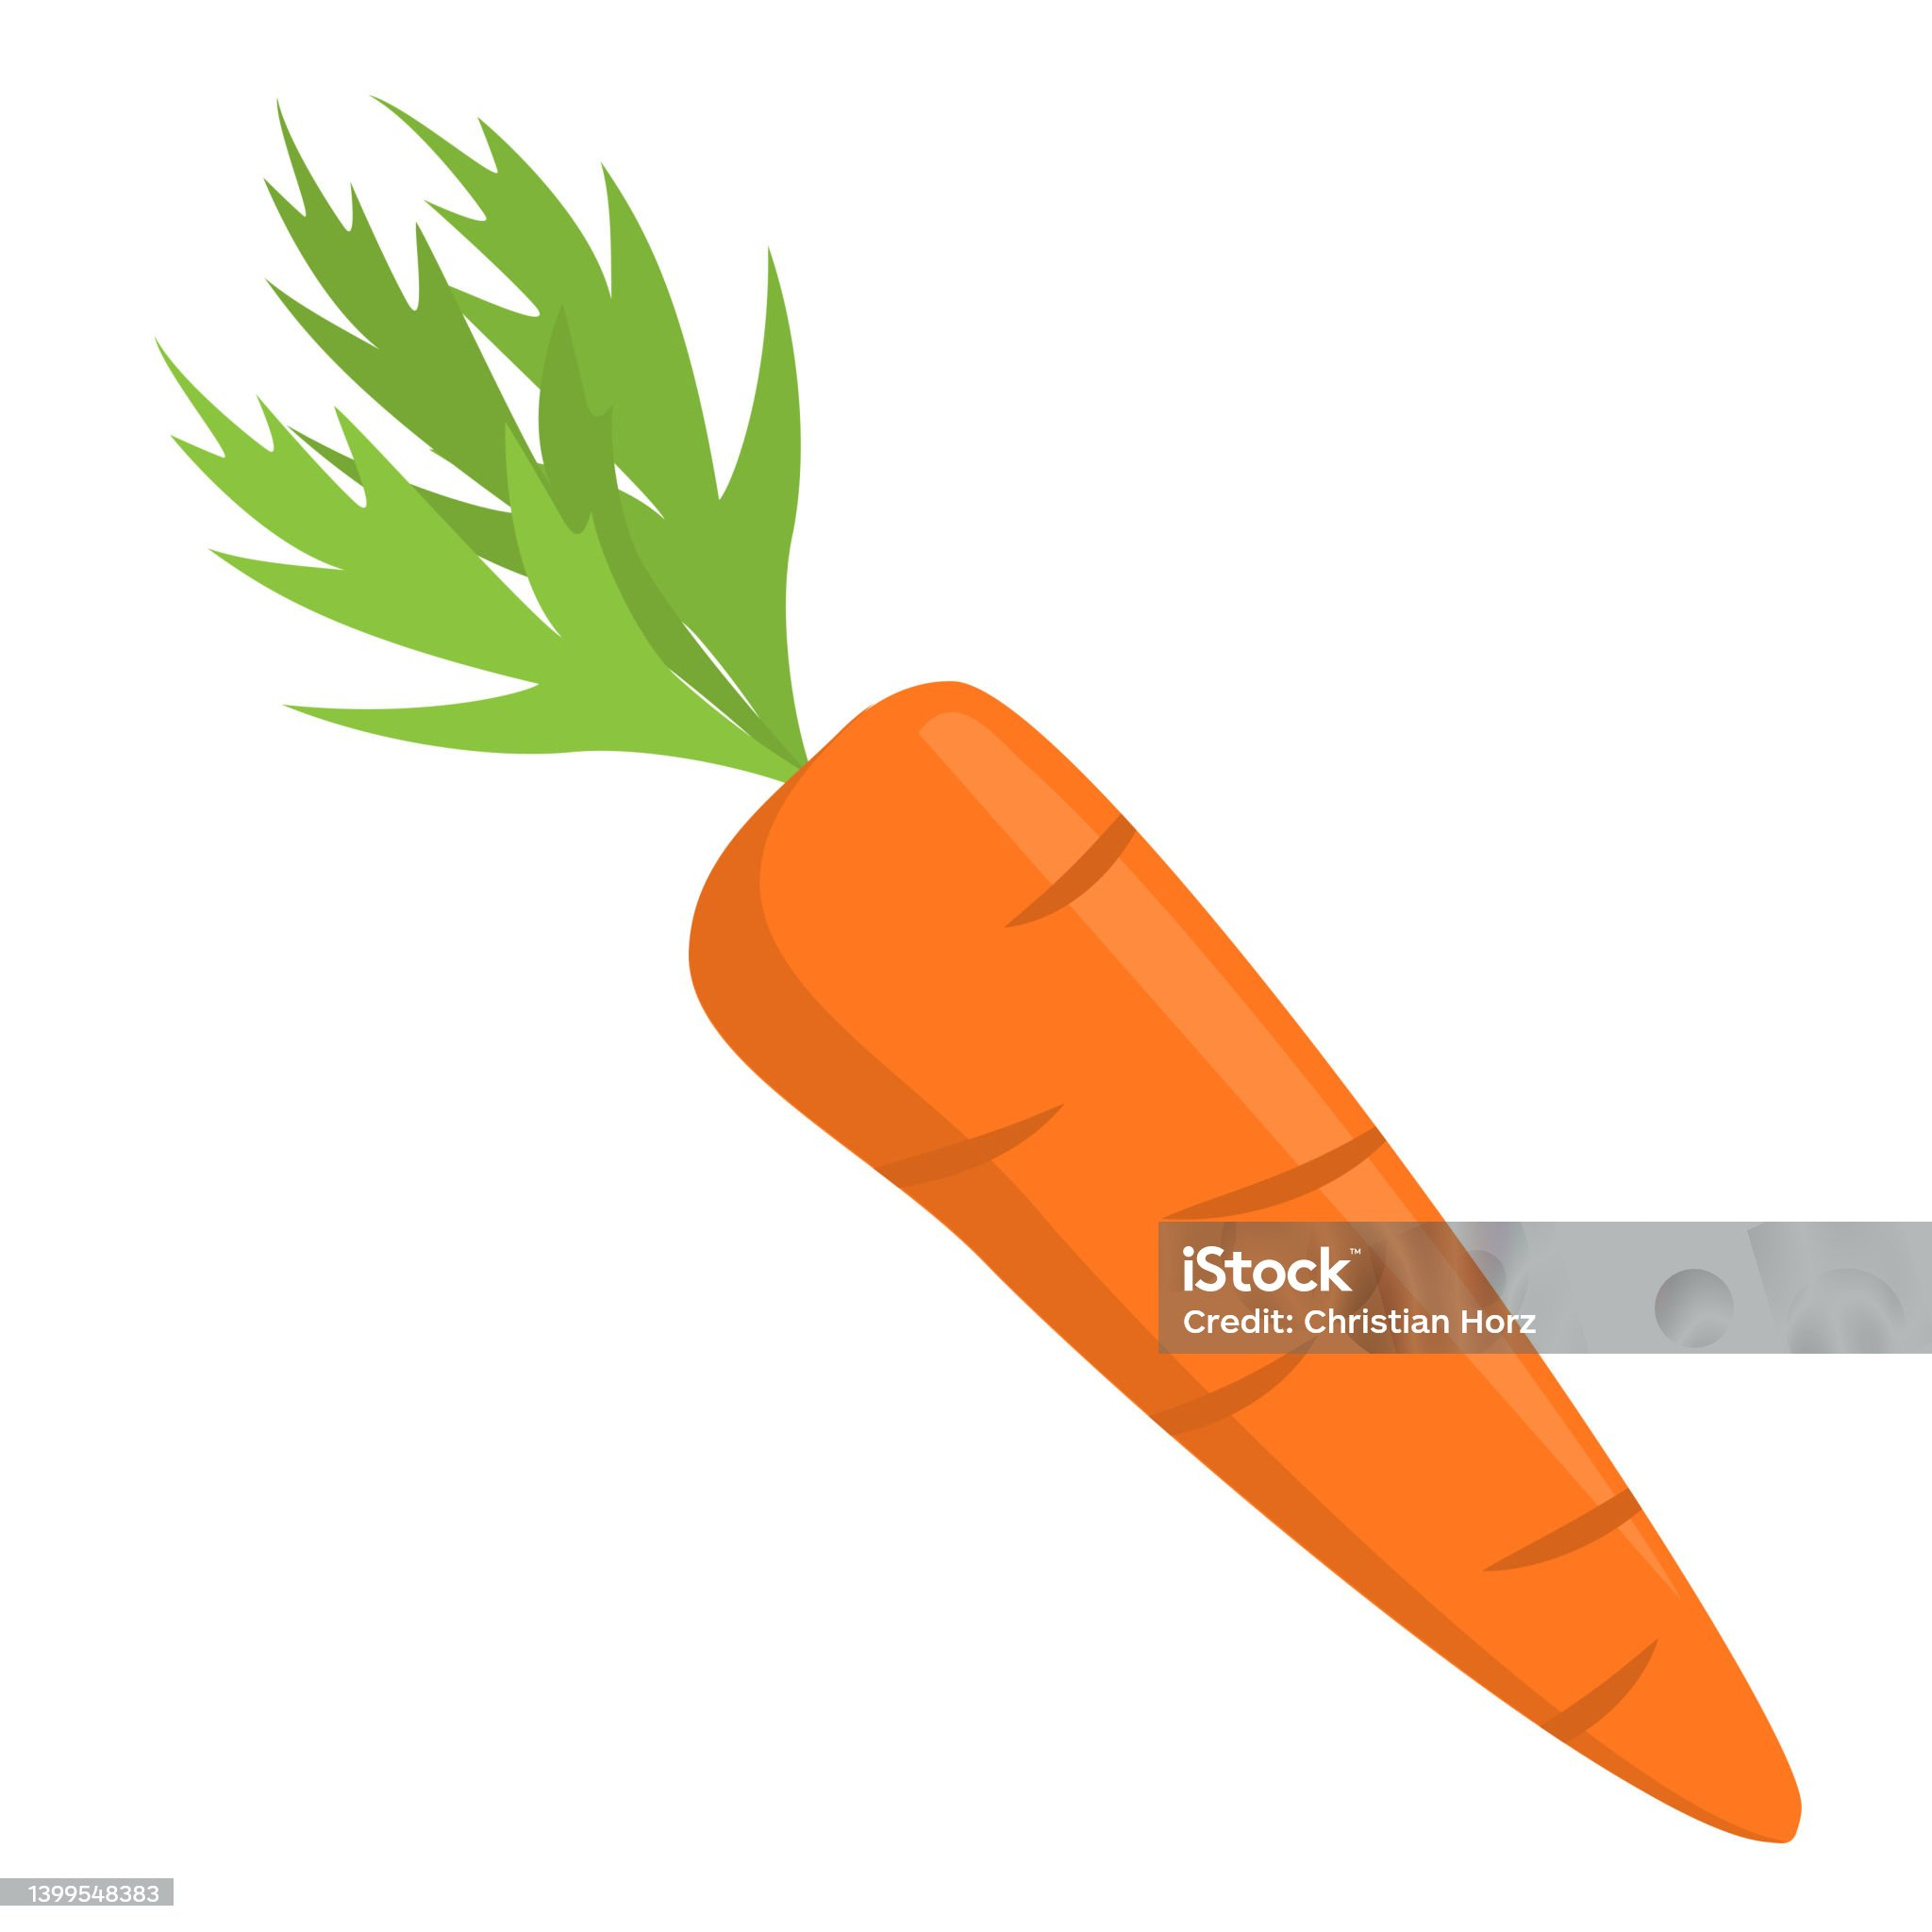
\includegraphics[scale=0.2]{Images/aaa.jpg}
		\caption{تغذیه سری موازی} % subcaption
		\label{fig14}
	\end{subfigure}
	\caption{}
\end{figure}


در این روش که برای تقسیم توان به توان‌های
$ 2^n$
 (یعنی ۲، ۴، ۸، ۱۶ و ...) استفاده می‌شود، تقسیم توان با استفاده از خطوط تغذیه باریک‌شونده
\LTRfootnote{Tapered Lines}
 مطابق شکل زیر انجام می‌شود تا امپدانس المان‌های پَچ (معمولاً ۱۰۰ اهم) را به امپدانس ورودی استاندارد (۵۰ اهم) تطبیق دهد.



\begin{figure}
	\centering
	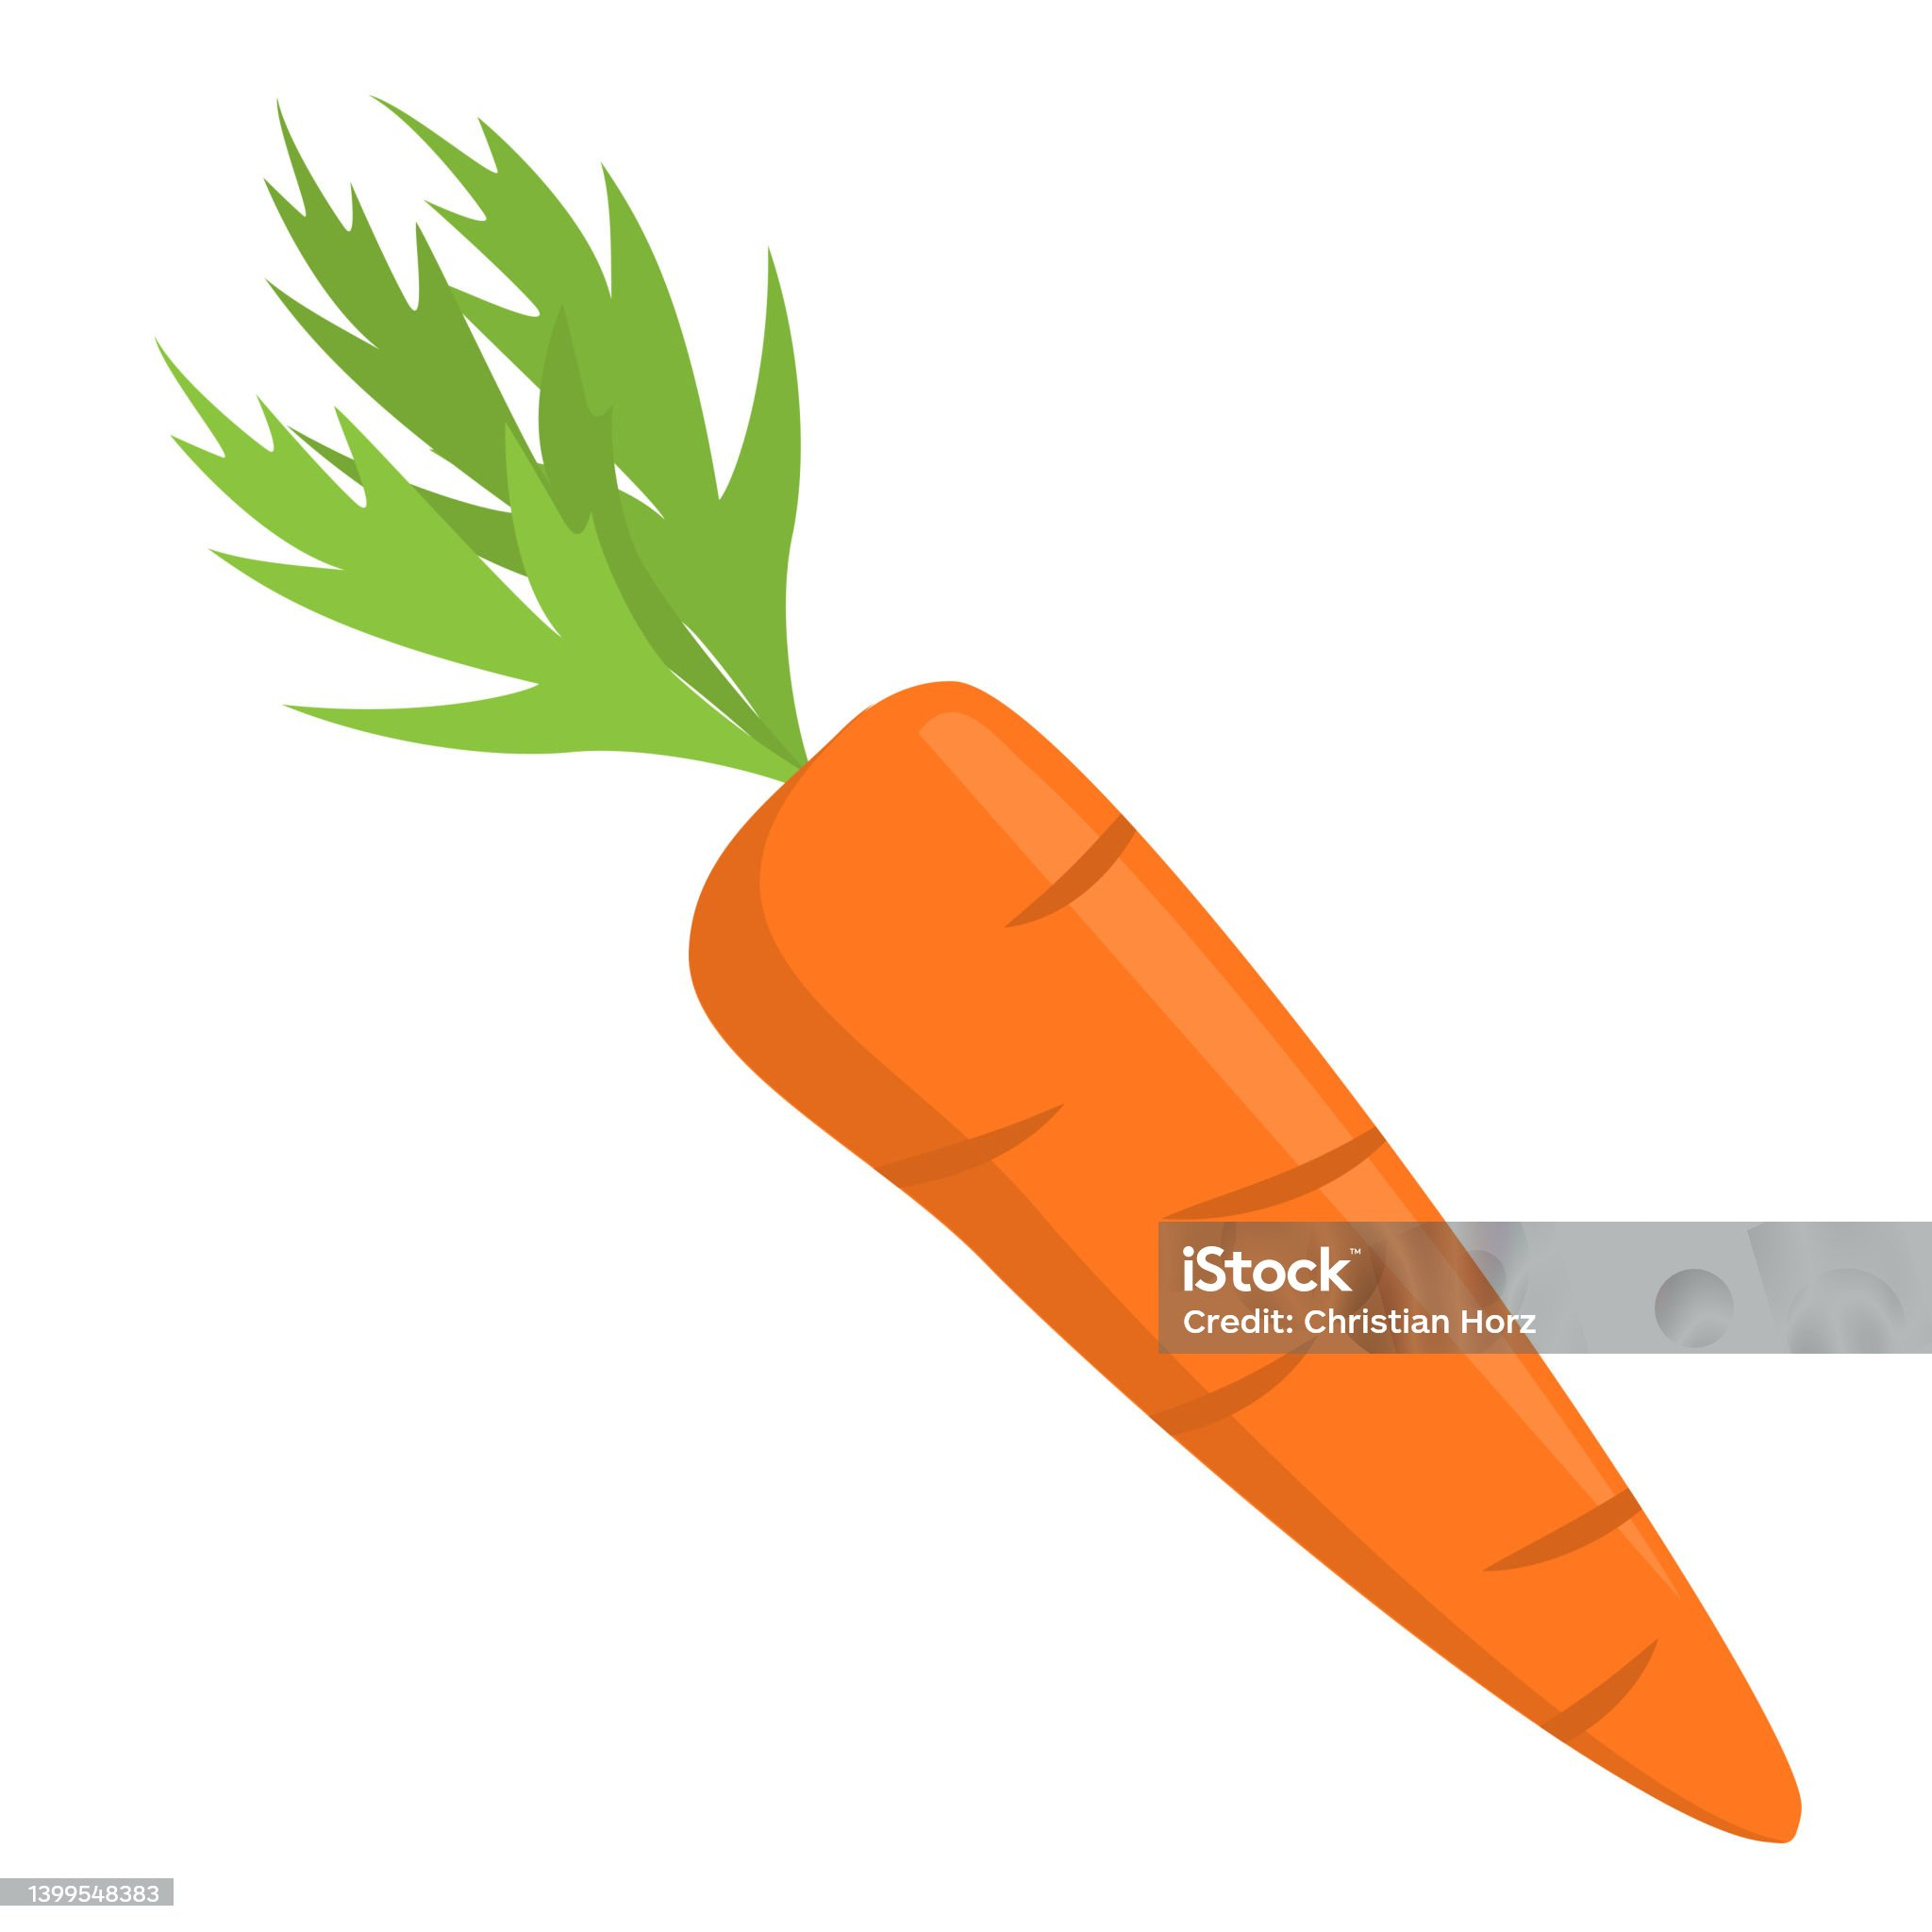
\includegraphics[scale=0.3]{Images/aaa.jpg}
	\caption{خطوط باریک شونده}
	\label{fig15}
\end{figure}

به علاوه میتوان با مبدل های امپدانس ربع طول موج هم این کار را انجام داد:
\begin{figure}
	\centering
	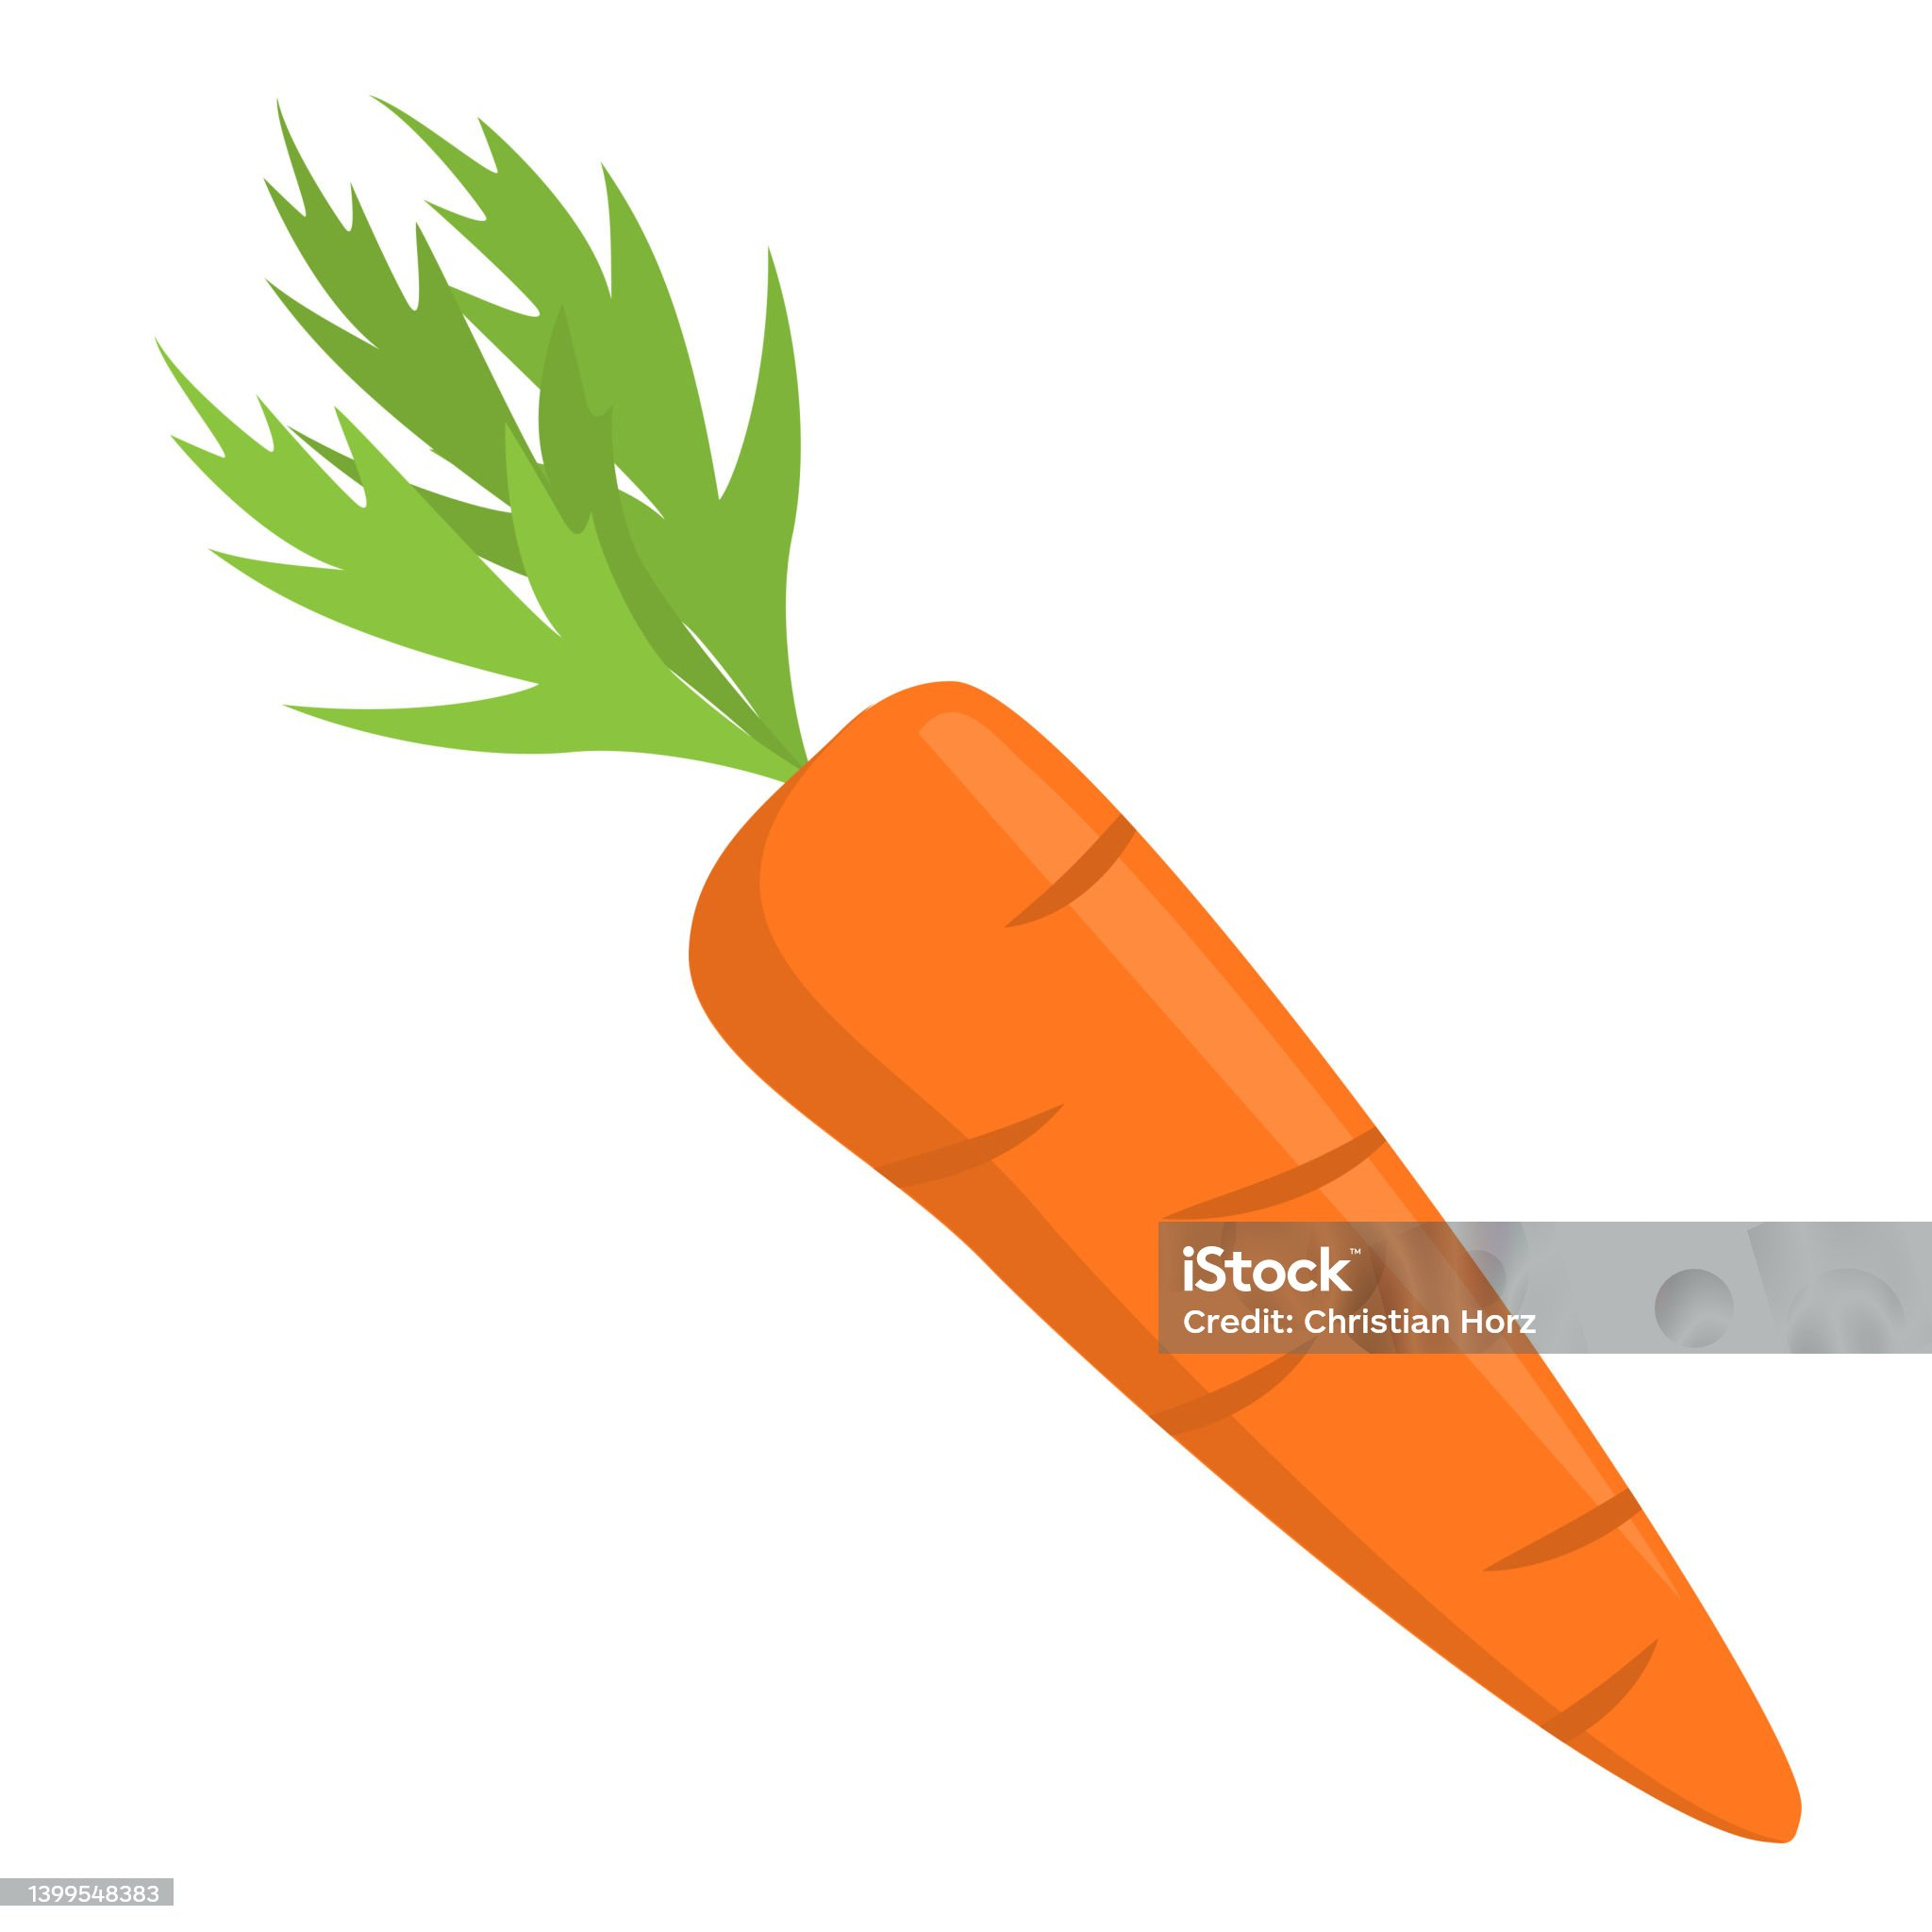
\includegraphics[scale=0.3]{Images/aaa.jpg}
	\caption{مبدل یک چهارم طول موج}
	\label{fig16}
\end{figure}

آرایه‌های تغذیه سری را می‌توان به راحتی با استفاده از مدل چاپی نوری برای المان‌های تشعشعی و شبکه تغذیه ساخت. البته این روش به آرایه با پرتو ثابت یا آرایه‌هایی که با تغییر فرکانس اسکن می‌شوند محدود می‌شود، ولی می‌توان از این تکنیک برای آرایه‌های خطی صفحه‌ای با پلاریزاسیون تکی یا دوگانه استفاده کرد. همچنین هرگونه تغییر در یکی از المان‌ها یا خطوط تغذیه، عملکرد بقیه را تحت تأثیر قرار می‌دهد. بنابراین در یک طراحی، در نظر گرفتن این اثرات و سایر اثرات مانند تلفیق متقابل و بازتابش‌های داخلی مهم است.


آرایه‌های تغذیه مشارکتی، متداول و دارای کاربردهای متنوعی هستند. با این روش، طراح کنترل بیشتری روی تغذیه هر المان (دامنه و فاز) دارد و این روش برای آرایه‌های فاز اسکن‌کننده، آرایه‌های چندپرتوئی یا آرایه‌های با پرتو شکل‌داده‌شده، ایده‌آل است. فاز هر المان را با استفاده از شیفت‌دهنده‌ها می‌توان کنترل کرد و دامنه را با استفاده از تقویت‌کننده‌ها و تضعیف‌کننده‌ها می‌توان تحت کنترل قرار داد.


نکته قابل توجه این است که چه در تغذیه سری و چه در مشارکتی، تشعشع از خط تغذیه قابل ملاحظه و مهم است که پلاریزاسیون را متقاطع و سطح لوب کناری آرایه را افزایش می‌دهد. که هر دو را می‌توان با جداسازی شبکه تغذیه از صفحه تشعشع‌کننده آرایه بهبود بخشید که این کار را می‌توان با استفاده از تغذیه‌های پروبی یا تغذیه روزنه‌ای انجام داد.


\section{تزویج}
یکی از مسائل مهم در طراحی آرایه‌های آنتنی، تزویج متقابل میان عناصر آرایه است. هنگامی که المان‌ها در فاصله‌ای کمتر از چندین طول‌موج قرار گیرند، میدان‌های الکترومغناطیسی هر المان بر سایر المان‌ها اثر می‌گذارد. این پدیده باعث می‌شود که جریان‌های القاشده روی المان‌های مجاور تغییر کنند و در نتیجه امپدانس ورودی، بهره و الگوی تابش کل آرایه دچار تغییر شود.


این تزویج باعث بوجود آمدن تغییرات زیر میشود : 

\begin{itemize}
	\item{
	انحراف امپدانس ورودی از مقدار طراحی شده
	} 
	\item{
	کاهش بهره و بازدهی آرایه
	}
	\item{
	تغییر در الگوی تشعشعی (افزایش
	\lr{sidelobe}
	ها).
	}
	\item{
	محدودیت پهنای باند عملیاتی.
	}
\end{itemize}

دو نوع چیدمان برای پَچ‌های میکرواستریپ وجود دارد: یکی در راستای محور
$ y$
 و دیگری در راستای محور
 $ x$
 (شکل
 \ref{fig17}).

هدف از میدانی که با تنظیم خطوط تغذیه در طول
$ y$
 قرار داده می‌شوند، این است که میدان‌های الکتریکی تشعشعی در تشدید در طول
 $ L$،
  پلاریزاسیون خطی ایجاد کند. 


این بدین معنی است که میدان‌های الکتریکی تشعشع‌یافته در طول
$ y$
 بیشتر پلاریزه می‌شوند و این نیز به معنای تزویج بیشتر در این وضعیت است. در نتیجه، این وضعیت نشان می‌دهد که چیدمان پَچ در طول محور
 $ x$،
  تزویج متقابل
\LTRfootnote{Mutual Coupling}
 را کاهش می‌دهد.
 
\begin{figure}
	\centering
	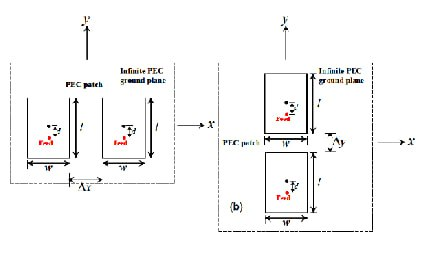
\includegraphics[scale=1]{Images/fig17.jpg}
	\caption{قرار گیری پچ ها در راستای 
		$x$ 
		و 
		$y$}
	\label{fig17}
\end{figure}

میتوان نشان داد که تزویج بین دو پچ تابع مکان یکی نسبت به دیگریست. برای این امر به مقاله ی
\cite{carver1981microstrip}
 استناد میکنیم. در این مقاله ثابت شده که با افزایش فاصله بین دو پچ ، تزویج متقابل نیز کاهش میابد. 

\begin{figure}
	\centering
	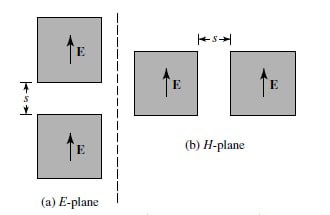
\includegraphics[scale=1]{Images/fig18.jpg}
	\caption{آرایش صفحه های E و H آنتن های مایکرواستریپ}
	\label{fig18}
\end{figure}

در نمودار 
\ref{fig19}
 تغییرات تزویج متقابل بین دو پچ در فواصل مختلف در دو آرایش E و H از مقاله ی 
 \cite{carver1981microstrip}
  نمایش داده میشود. 

\begin{figure}
	\centering
	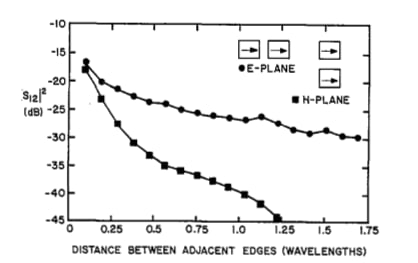
\includegraphics[scale=1]{Images/fig19.jpg}
	\caption{نمودار تزویج متقابل بین دو پچ در آرایش E و H}
	\label{fig19}
\end{figure}

در شکل فوق ابعاد آنتن به صورت زیر میباشد:
\begin{align}
	\label{eq:eq8}
	W = 10.57 \text{cm}, L = 6.55 \text{cm}, h = 0.1588 \text{cm}, \varepsilon_r = 2.55, f_r = 1.410 \text{MHz}
\end{align}

ابعاد
$ L$
 و
 $ W$
  از فرمول های 
  \ref{eq:eq9}
   تبعیت میکنند:
\begin{align}
	\label{eq:eq9}
	W = \frac{c}{2f_r\sqrt{\frac{\varepsilon_r+1}{2}}}
\end{align}
که در آن:
\begin{itemize}
	\item{$W$:
	عرض پچ(بر حسب متر)
	}
	\item{$c$:
	سرعت نور در خلاء
	}
	\item{$f_r$:
	فرکانس رزونانس (بر حسب هرتز)
	}
	\item{$\varepsilon_{r}$:
	ثابت دی الکتریک نسبی زیرلایه
	}
\end{itemize}


\begin{align}
	\label{eq:eq10}
	\varepsilon_{\text{eff}} = \frac{\varepsilon_R+1}{2} + \frac{\varepsilon_R-1}{2}\left[\frac{1}{\sqrt{1+12\left(\frac{h}{W}\right)}}\right]
\end{align}

\begin{align}
	\label{eq:eq11}
	\text{Length} = \frac{c}{2f_0\sqrt{\varepsilon_{e}}} - \left(2 \times \left[0.412h\frac{(\varepsilon_{e}+0.3)\left(\frac{W}{h}+0.264\right)}{(\varepsilon_{e}-0.258)\left(\frac{W}{h}+0.8\right)}\right]\right)
\end{align}

که با جایگذاری به تقریبا به همین اعداد میرسیم.


در تزویج بین دو پَچ مستطیلی، اگر المان‌ها هم‌راستا در صفحه E باشند، این آرایش، آرایش صفحه E نامیده می‌شود و اگر هم‌راستا در صفحه H باشند، این آرایش، آرایش صفحه H نام خواهد گرفت.

در آرایش صفحه E، معمولاً برای فواصل بسیار کوچک(
$s < 0.10\lambda$)،
 بیشترین تزویج را نشان می‌دهد، در حالی که در آرایش صفحه H، معمولاً برای فواصل بزرگ(
 $s > 0.10\lambda$)،
  کمترین تزویج را نشان می‌دهد. فاصله‌ای که در آن تزویج یک صفحه از دیگری پیشی می‌گیرد، به خواص الکتریکی و ابعاد هندسی آنتن مایکرواستریپ بستگی دارد.

به طور کلی، تزویج متقابل بیشتر به میدان‌هایی که در امتداد فصل‌مشترک هوا با دی‌الکتریک وجود دارند مربوط میشود. این میدان ها میتوانند به امواج فضایی(با تغییرات شعاع
$1/\rho$)
امواج مرتبه بالاتر(با تغییرات شعاع
$1/\rho^2$)
امواج سطحی(با تغییرات شعاع
$1/\rho^{\frac{1}{2}}$)
وامواج نشطی(با تغییرات شعاع
$\exp{-\lambda_{p}/\rho^{\dfrac{1}{2}}}$)
تجزیه شوند. به دلیل تغییرات شعاعی کروی، امواج فضایی و مرتبه بالاتر برای فواصل کوچک و امواج سطحی برای فواصل بزرگ غالب می‌شوند.


امواج سطحی که داخل دی‌الکتریک وجود دارد، در آن منتشر می‌شود و تحریک آن‌ها تابعی از ضخامت دی‌الکتریک است. برای یک پَچ مستطیلی، میدان‌ها در جهت انتشار در امتداد صفحه E از نوع TM و در امتداد صفحه H از نوع TE هستند. در آرایش صفحه E، همانطور که در شکل فوق نشان داده شده، المان‌ها در راستای صفحه E قرار دارند و در فاصله بین المان‌ها میدان از نوع TM است. یک تحریک موج سطحی قوی‌تر بین المان‌ها وجود دارد و تزویج بزرگتر است. اما در صفحه H این گونه نیست و تحریک موج سطحی قوی وجود ندارد و تزویج کمی وجود دارد. با افزایش ضخامت زیرلایه که باعث تحریک موج سطحی TE مرتبه بالاتر می‌شود، این تزویج تغییر می‌کند.





























